\documentclass[12pt,openright]{book}

\usepackage{newtxtext}
\usepackage[utf8]{inputenc}
\usepackage{lipsum}
\usepackage{lineno}

%%%%%%%%%%%%%%%%%%%%%%%%%%%%%%%%%%%%%%%%%%%%%%%%%%%%%%%%%%%%%%%%%%%%%%%%
%\usepackage{fontspec}
%\setmainfont{Times New Roman}
%\setsansfont{Arial}
%\setmonofont{Gill Sans MT}

%\usepackage{xeCJK}
%\setCJKmainfont[BoldFont={Microsoft YaHei},ItalicFont={STKaiti}]{SimSun}
%\setCJKsansfont[BoldFont={Microsoft YaHei},ItalicFont={STKaiti}]{STKaiti}
%\setCJKmonofont[BoldFont={STZhongsong},ItalicFont={STZhongsong}]{STZhongsong}

%\setCJKmainfont[BoldFont={FZHei-B01},ItalicFont={FZKai-Z03}]{FZShuSong-Z01}
%\setCJKsansfont[BoldFont={FZHei-B01},ItalicFont={FZHei-B01}]{FZHei-B01}
%\setCJKmonofont[BoldFont={FZHei-B01},ItalicFont={FZHei-B01}]{FZFangSong-Z02}

%%%%%%%%%%%%%%%%%%%%%%%%%%%%%%%%%%%%%%%%%%%%%%%%%%%%%%%%%%%%%%%%%%%%%%%%

%\usepackage[14pt]{extsizes} % use this when fontsize is not 10, 11 or 12pt
\usepackage{geometry}
\geometry{a4paper,inner=3cm,outer=2.54cm,top=2.54cm,bottom=2.54cm}

\usepackage{fancyhdr}
\renewcommand{\headrulewidth}{0pt}

\fancypagestyle{fancy-stylename}{
\fancyhf{} % clear header/footer settings
\fancyhead[LE,RO]{\textit{Guides and tutorials}}
\fancyhead[RO]{\itshape\nouppercase{\leftmark}}
\fancyfoot[OR,EL]{\thepage}}

\fancypagestyle{plain}{
\fancyhf{}
\fancyfoot[OR,EL]{\thepage}}

%\renewcommand{\headrulewidth}{0pt}
%\renewcommand{\footrulewidth}{1pt}
%\rhead{\leftmark}
\pagestyle{fancy-stylename}
\AtBeginDocument{\addtocontents{toc}{\protect\thispagestyle{empty}}}

\usepackage{titlesec}
%\titleformat{\chapter}{\normalfont\huge\bfseries}{}{0pt}{\Huge}
%\titleformat{\chapter}[display]{\normalfont\huge\bfseries}{\chaptertitlename\ \thechapter}{20pt}{\Huge}

%\titleformat{\chapter}[hang]{\normalfont\huge\bfseries}{}{0pt}{\Huge\thechapter.\;}{\Huge}

\titleformat{\chapter}[hang]{\normalfont\huge\bfseries}{\Huge\thechapter. \,}{0pt}{\Huge}

% \usepackage{etoolbox}

\renewcommand\chaptermark[1]{\markboth{#1}{}}

%\usepackage{anyfontsize}
%\usepackage{newtxtext}\textbf{}
%\usepackage{mathpazo}

\usepackage{amsmath}
\usepackage{chemformula}
\usepackage{gensymb} % for degree symbol \ang{90} or use the following line
%\usepackage{siunitx} % then use 90\si{\degree} in the document
% $^{\circ}$ is another way of obtaining roughly the right symbol

\usepackage[titles]{tocloft}
\renewcommand{\cftchapleader}{\cftdotfill{\cftdotsep}} % for chapters
%\renewcommand{\cftsecleader}{\cftdotfill{\cftdotsep}} % for sections
%\title{\bfseries \fontsize{80}{100}\selectfont PhD Thesis title}
%\title{\bfseries\sffamily PhD Thesis title}
%\title{\bfseries\textsf PhD Thesis title}
% \title{\Huge {\bfseries \LaTeX\ Thesis template}}
% \author{Author name}
% %\date{\today}
% %\date{2019/12/15}
% \date{Dec. 21, 2019}

\renewcommand{\baselinestretch}{1.5}
%\setlength{\parskip}{1em}

\usepackage{hyperref}
\hypersetup{hidelinks} % or
% \hypersetup{pdfborder={0 0 0}}

%\renewcommand{\bibname}{}

\usepackage{longtable}
\usepackage{lscape}
\usepackage{graphicx}
\usepackage[labelfont=bf]{caption}

\graphicspath{ {figure/} }
\usepackage{array}

\usepackage[flushleft]{threeparttable}
\usepackage{multirow}
\usepackage{booktabs}

%\usepackage{layout}
%\usepackage{showframe}
%\the\textwidth = 438.74153pt --> 6.09363236111 in, 1828.08970833 px for full textwidth 300 dpi pic
%% resample the figure pixel to \textwidth in inches * 300 pixels wide
% \usepackage{layout}
% \usepackage{showframe}


\usepackage{listings}
\renewcommand{\ttdefault}{cmtt}
\lstdefinestyle{estyle}{
  basicstyle=\ttfamily \lst@ifdisplaystyle\small\fi
}

\lstset{language=[LaTeX]TeX,
	   style=estyle,
	   texcsstyle=*\color{blue},
	   keywordstyle=\color{blue},
	   lineskip={-1.5pt},
	   morekeywords={frontmatter,mainmatter}
}
\usepackage[shortlabels,inline]{enumitem}
\setlist{nolistsep}

\begin{document}
% \the\textwidth

\begin{titlepage}
%\maketitle
%\thispagestyle{empty}
\begin{center}
  \vspace*{1cm}

  \Huge \textbf{Thesis Title}

  \vspace{0.5cm}

  \Large{Thesis subtitle}

  \vspace{2cm}

  \large{Inaugural-Dissertation \\ to obtain the academic degree \\ Doctor rerum naturalium (Dr. rer. nat.)}

  \vspace{1.5cm}

  \large{submitted to the Department of xxxBCPxxx \\ of XXX University}

  \vspace{1.5cm}

  %\textbf{Author Name}

  \vfill

  \large{by \\ \textbf{San Zhang} \\ from Beijing, China}
  
  \vspace{0.5cm}

  \large{2020}
  
  % A thesis presented for the degree of Doctor of Philosophy \\
  % Department name \\
  % University name \\
  % Date

\end{center}
\end{titlepage}

\pagestyle{empty}
\tableofcontents
\clearpage

\pagestyle{fancy-stylename}

\frontmatter
%\pagenumbering{roma}  % Roman page number for toc
%\setcounter{page}{2} % Make it start with "ii"

\chapter*{Acknowledgements}
\addcontentsline{toc}{chapter}{Acknowledgements}
\lipsum[1-5]

\chapter*{List of Abbreviations}
\addcontentsline{toc}{chapter}{List of Abbreviations}

\begin{tabular}{p{0.15\textwidth}p{0.3\textwidth}||p{0.01\textwidth}p{0.15\textwidth}p{0.3\textwidth}}
  \multicolumn{2}{l}{\textbf{Commonly used characters}}
  & & \multicolumn{2}{l}{\textbf{Commonly used characters}}\\
  \S & \lstinline|\S| & & \dag & \lstinline|\dag| \\
  \ddag & \lstinline|\ddag| & & \P & \lstinline|\P| \\
  \copyright & \lstinline|\copyright| & & \textregistered & \lstinline|\textregistered| \\
  \texttrademark & \lstinline|\texttrademark| & & \pounds & \lstinline|\pounds| \\
  \textbullet & \lstinline|\textbullet| & &\& &  \lstinline|\textbackslash|   \\
\end{tabular}

\newpage

\chapter*{Abstract}
\addcontentsline{toc}{chapter}{Abstract}

Lorem Ipsum is simply dummy text of the printing and typesetting industry. Lorem Ipsum has been the industry's standard dummy text ever since the 1500s, when an unknown printer took a galley of type and scrambled it to make a type specimen book. It has survived not only five centuries, but also the leap into electronic typesetting, remaining essentially unchanged. It was popularised in the 1960s with the release of Letraset sheets containing Lorem Ipsum passages, and more recently with desktop publishing software like Aldus PageMaker including versions of Lorem Ipsum.~\cite{Weir04}

The command \lstinline|\pagenumbering{roman}| will set the page numbering to lowercase Roman numerals. Following command is used to set the layout of the page number.

\lstinline|\pagenumbering{num_style}|

Below, a list of styles available for page numbering:
\begin{itemize}[label=\labelitemii]
  \item arabic: arabic numerals
  \item roman: lowercase roman numerals
  \item Roman: uppercase roman numerals
  \item alph: lowercase letters
  \item Alph: uppercase letters
\end{itemize}

In books, is customary to use Roman numerals for the pages before the first chapter/section, and Arabic numbers for the rest of the document. The commands that control the page numbering are: \lstinline|\frontmatter|, the pages after this command and before the command \lstinline|\mainmatter|, will be numbered with lowercase Roman numerals. \lstinline|\mainmatter|, this will restart the page counter and change the style to Arabic numbers.

The information displayed in the footer and the header of a document depends on the page style currently active, these page styles are more notorious in the \textbf{book} document class:

The selectors that can be passed, inside brackets, to the commands \lstinline|\fancyhead| and \lstinline|\fancyfoot| are:
\begin{itemize}
  \item E: for even page
  \item O: for odd page
  \item L: for left side  
  \item C: for centered
  \item R: for right side
\end{itemize}

\centerline{\rule{0.95\textwidth}{0.5pt}}


Starting New Lines and New Pages:

This will be on one line, between lines the space is 10pt here. \\[10pt] this will be on the next line. 

To force a new page, the simplest command is \lstinline|\newpage|, which starts a new page immediately. There is also the command \lstinline|\clearpage|, which acts like \lstinline|\newpage| except that it also forces any leftover figures or tables to print before starting the new page. With the twoside documentclass option, the command \lstinline|\cleardoublepage| produces a blank page, if necessary, to ensure that the new page starts on a new sheet of paper.

The commands \lstinline|\hspace| and \lstinline|\vspace| leave horizontal and vertical space in your text. Both commands take a mandatory parameter—the amount of blank space you want to leave. For example, \lstinline|\vspace{3in}| will leave 3 inches of blank space in your text. If vertical space is requested in the middle of a paragraph, the space will appear after the current line has ended.

This text starts at the left margin\\
\hspace*{1in}This text starts a new line after a one-inch space

To draw a line (horizontal or vertical) on the page, use the \lstinline|\rule| command:
\begin{lstlisting}
  \rule[lift]{width}{height}
\end{lstlisting}
\lstinline|width| is the horizontal dimension, \lstinline|height| is the vertical dimension, and the optional parameter lift is the amount raised above the baseline. For example, the line below was drawn with the command \lstinline|\rule{0.95\textwidth}{1pt}|.

\rule{0.95\textwidth}{1pt}

The command \lstinline|\footnote{footnote text}| should be placed exactly where you want the footnote number to appear, with no extra space between the \lstinline|\footnote| command and the text before it. For example: 

This is text with a note. \footnote{This is the note text. Here it is at the bottom of the page.}

\mainmatter
%\pagenumbering{arabic} % Start text with arabic 1
\chapter{Title of Chapter One}

\LaTeX{} input files have names end with the extension \lstinline{.tex}. Normal \LaTeX{} document can be divided into two parts: the preamble and the document text. The part of your .tex file before the \lstinline|\begin{document}| command is called the \textbf{preamble}. In the preamble, you can define the type of document you are writing and the language, load extra packages you will need, and set several parameters. 

\begin{lstlisting}
\documentclass[options]{class}

% preamble settings

\begin{document}

Document text
  
\end{document}
\end{lstlisting}


\textbf{Commands} produce text or space. For example, \lstinline|\hspace{2in}| and \lstinline|\vspace{2in}| are commands that create 2 inches of horizontal and vertical space respectively, and \lstinline|\textit{}| will create \textit{some italic words} puts the contents of its argument in italic type. Many commands take arguments, either mandatory or optional; some commands, like \lstinline|\today| don’t.

\textbf{Mandatory arguments} supply information required for a command to execute. For
example, \lstinline|\hspace{2in}| needs the information provided by the argument to generate the horizontal space. Mandatory arguments are enclosed in braces: \{\}.

\textbf{Optional arguments} are allowed on some commands and are enclosed in square brackets: []. For example, the size of type to be used for your main text is an optional argument in the \lstinline|\documentclass| command. To use the article class in 11-point type, you would type \lstinline|\documentclass[11pt]{article}|. Without this optional argument, you would get the default 10-point type.

\textbf{Declarations} produce neither text nor space, but either affect the way \LaTeX\ prints the following text or provide information for later use. Font size changes are an example of declarations. \lstinline|\large{}| will cause any text that follows to appear in a larger type size. Declarations are often used within a group to limit their scope. For example: {\large Only the text inside these braces will be large.}


\textbf{Environments} are blocks of text that receive special processing. An environment is defined by a matching  \lstinline|\begin{environment name} ... \end{environment name}|. An environment is also a group, in the same way that a pair of braces delimits a group. For example, a quotation might be formatted as follows:

\begin{quote}
  \small This text is set off from surrounding text and indented from both margins. The font size of this quotation will be smaller because of the "small" command inside the quote environment.
\end{quote}

Note that a blank line before an environment ends the previous paragraph. A blank line following an environment indicates that the next line starts a new paragraph. Environments can be nested, i.e., the first started is the last ended.

* Some commands can have a * appended to the name, which indicates a variation on a command or environment. For example, \lstinline|\\| indicates a line break. \lstinline|\\*| indicates a line break with the restriction that \LaTeX\ is not allowed to begin a new page at that point. Space printed by \lstinline|\vspace| and \lstinline|\hspace| commands is normally dropped if it appears at the beginning or end of a line or page. If you want the space printed no matter where it falls, you would use \lstinline|\hspace*| or \lstinline|\vspace*|. Normally, section headings are automatically numbered, but \lstinline|\section*{My Heading}| will produce an unnumbered section heading.

These four classes are single-spaced by default, and have 10, 11, and 12-point type sizes available as options. 10 points is the default size.

The slides class uses sans-serif type fonts much larger than the usual ones and expects the document to be divided up into 1-page sections.

\section{1.1 Title}

A document class may be modified by options, which are placed in square brackets after the \lstinline|documentclass| command. Multiple options are separated by commas: \lstinline[breaklines]|\documentclass[option1,option2]{class}|.

The standard class options include:
\begin{description}
  \item[10pt, 11pt, 12pt] Selects the point size of main font for the document. If no option is specified, 10pt is assumed. This document uses 12-point type.
  \item[twocolumn] Produces two-column pages.
  \item[titlepage] Causes the \lstinline|maketitle| command to generate the title page on a separate page for the article class. This option is not necessary for the book and report classes, as they print separate title pages by default.
  \item[leqno] Puts equation numbers on left side. (They are on the right by default.)
  \item[fleqn] Left-aligns equations. (They are centered by default.)
  \item[twoside] Formats for printing on both sides of paper. (Whether the document is actually printed two-sided depends on the printer.) Twoside is the default for the \textbf{book} class, but not for any of the other classes.
  \item[openright] If the twoside option is in effect, chapters will begin on right hand pages. This is the default for the \textbf{book} class. It does not apply to the article class, which does not contain chapters. (The opposite of \textbf{openright} is \textbf{openany}.)
\end{description}


The auxiliary files have the same “root” name as the \LaTeX{} input file, but different extensions. For example, all documents need an AUX file. If the input file is named myfile.tex, the AUX file will be named myfile.aux. Other auxiliary files (see the list below) are needed only if you are producing a table of contents, etc. Auxiliary files are created automatically as they are needed.

\begin{itemize}[label=\labelitemii]
\item filename.aux : always needed
\item filename.toc : for table of contents
\item filename.lot : for list of tables
\item filename.lof : for list of figures
\end{itemize}

If you have only one line to center, it’s easier to use the plain \TeX{} command
\lstinline|\centerline|; for example, \lstinline|\centerline{This line will be centered}| produces: \par
\centerline{This line will be centered}

If you have several lines to be centered horizontally, the center environment is convenient. The example below produces three lines, each horizontally centered.
\begin{center}
  This is line one. \\
  This is line two. \\
  This is line three.
\end{center}

\subsection{1.1.1 title}

The quote environment begins a new line and indents text from both sides. It is delimited with \textbackslash begin\{quote\} and \textbackslash end\{quote\}. Any special effects (such as changes to the type size or style) started within the quote environment
are terminated by \textbackslash end\{quote\}. New paragraphs are block style: that is, no indent and a blank line as separation. This section is inside a quote environment. There is also a very similar environment called quotation. The only difference is that paragraphs in the quotation environment are indented with no blank line between.

\subsection{1.1.2 title}

This example shows how to cite within the figure caption, see in Figure~\ref{fig:captioncitation}.

\begin{figure}[htp]
	\centering
	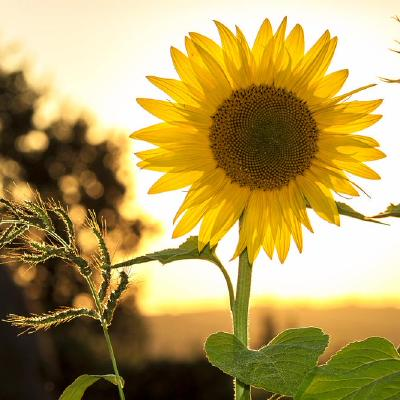
\includegraphics[width=\textwidth]{29571453}
	\caption[figure caption with citation.]{figure caption with citation.~\cite{ibge1993}} 
	\label{fig:captioncitation}
\end{figure}

\begin{figure}[htp]
  \centering
  \begin{tabular}{ll}
    A & B \\
    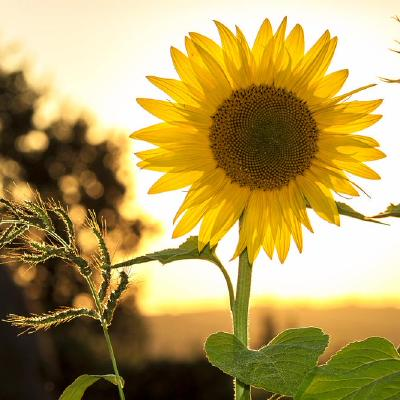
\includegraphics[width=0.45\textwidth]{29571453}
    & 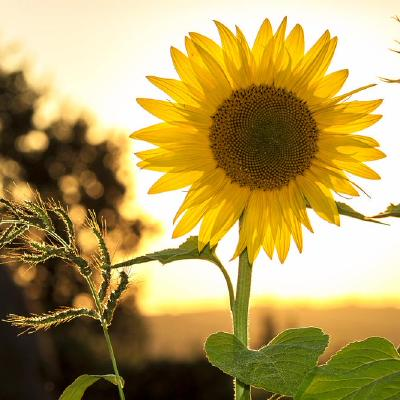
\includegraphics[width=0.45\textwidth]{29571453} \\
  \end{tabular}
  \caption[figure caption with citation.]{figure caption with } 
	\label{fig:figurespanel_table}
\end{figure}

\subsubsection{1.1.1.1 title won't show in the contents}

What if I also referenced the same reference here~\cite{ibge1993}, why?

\noindent The basic document type for \LaTeX\ is shown in Table \ref{tab:document type}.

\begin{table}[!htbp]
  \caption{Document Classes for \LaTeX}
  \label{tab:document type}
  \begin{tabular}{@{}lp{0.9\textwidth}@{}}
    \toprule
    \textbf{Document type} & \textbf{Description} \\
    \midrule
    article  &  For simple and short documents (journal articles, short reports). A good all-purpose class, the most commonly used. \\
    report & For longer documents and dissertations \\
    book & Useful to write books \\
    letter & For letters \\
    slides & For slides, rarely used \\
    beamer & Slides in the Beamer class format \\
    %See the beamer documentation for a better
    \bottomrule
  \end{tabular}
\end{table}
  
These classes provide preset formats with default margins paragraph formatting, and special commands suitable for producing specific sections. For example, the article, report, and book classes include a variety of commands to format section headings
(\lstinline|\part|, \lstinline|\chapter|, \lstinline|\section|, \lstinline|\subsection|, \lstinline|\subsubsection|, etc.), as well as commands to produce a title page and a table of contents. There are minor differences between these three classes. The book class, for example, uses a smaller printed page size—about 5×7.5 inches—and is formatted for two-sided printing by default. The article class is intended for shorter works and does not have chapters (so articles can be easily included in reports or books). The \textbf{letter} class provides special commands to produce the salutation, address, and closing.

%\vskip 0.1in
Sometimes you may want to change the style or size of text that is not a section heading. These commands can be combined, provided the font thus requested actually exists. For example, the command \textbackslash textbf\{\textbackslash textit\{This is bold italic\}\} produces: \textbf{\textit{This is bold italic}}.

\begin{center}
\begin{tabular}{|p{0.2\textwidth}p{0.25\textwidth}p{0.45\textwidth}|}
  \hline
  \textbackslash textit\{\} & \textit{italic} & Italic shape, used mostly for emphasis\\
  \textbackslash textsl\{\} & \textsl{slanted} & Slanted shape, a bit different from italic\\
  \textbackslash textsc\{\} & \textsc{SMALL CAPS} & Small caps shape, use sparingly\\
  \textbackslash textup\{\} & \textup{upright} & Upright shape, usually the default\\
  \textbackslash textbf\{\} & \textbf{boldface} & Boldface series, often used for headings\\
  \textbackslash textmd\{\} & \textmd{medium} & Medium series, usually the default\\
  \textbackslash textrm\{\} & \textrm{roman} & Roman family, usually the default\\
  \textbackslash textsf\{\} & \textsf{sans serif} & Sans Serif family, used for posters, etc.\\	
  \textbackslash texttt\{\} & \texttt{typewriter} & Typewriter family, fixed-pitch characters\\
  \textbackslash emph\{\} & \emph{emphasized} & Use for emphasis, usually changes to italic\\
  \textbackslash underline\{\} & \underline{underline} & Use for \underline{underline}\\
  \hline	
  \multicolumn{3}{p{0.9\textwidth}}{Use \textbackslash usepackage\{ulem\}, then \textbackslash uline\{emphasized\}, or \textbackslash emph\{for long sentence in order to change lines automatically.\}}
\end{tabular}
\end{center}

\dag\!\dag \, Here \textbackslash ! means negative distance. \dag\!\dag

The default document size is 10 points. Therefore \textbackslash normalsize means 10 points for a document in which no size option has been included. This document is printed in 12 points, so in this case, \textbackslash normalsize is 12 points. (Note that when normalsize is 12 points, there is no difference between huge and Huge. They are both the largest size—25 points.)

{\tiny tiny}

{\scriptsize scriptsize}

{\footnotesize footnotesize}

{\small small}

{\normalsize normalsize}

{\large large}

{\Large Large}

{\LARGE LARGE}

{\huge huge}

{\Huge Huge}

\paragraph{title won't show in the contents} 

Examples for chemical formula:

\vskip 0.1in

\ch{3 H2O} 

\ch{1/2 H2O} 

\ch{AgCl2-} 

\ch{H2_{(aq)}}

\vskip 0.1in

\subparagraph{title won't show in the contents}

% An extra wide table 
\begin{landscape}
  After this point, everything is displayed in landscape format.
  
  \begin{tabular}{|c|c|c|c|c|c|c|c|c|c|c|c|}
    \hline
    Year & 2000 & 2001 & 2002 & 2003 & 2004 & 2005 & 2006 & 2007 & 2008 & 2009 & 2010 \\
    \hline 
    GPD in billions & 235  &  225 bn & 223 bn & 323 & 423  & 523 & 624 & 725 & 826  & 924  & 1022  \\
    \hline 
  \end{tabular}
\end{landscape}

After this point, everything is displayed in portrait format.

\section{1.2 Title}

Since documents of any length are usually divided into sections, the classes article, report, and book have a set of commands which take the name of the section as an argument. The author uses these commands in the proper order, providing the section name, and LATEX takes care of formatting the headings (boldface, larger typesize, etc.) and numbering them appropriately. The sectioning commands are:

\textbf{\lstinline|part| \lstinline|section| \lstinline|paragraph|
\textbackslash chapter \textbackslash subsection \textbackslash subparagraph
\textbackslash subsubsection}

Note that the \textbackslash chapter command is not available in article class. The \textbackslash part heading is rarely used. In most document classes, headings made with the lowest level headings, \textbackslash paragraph and \textbackslash subparagraph are not numbered by default. You can make less formal headings by using the sectioning commands with a star (*) appended to the  command names listed above. In this case, the section headings will
not show up in the table of contents and will not be numbered.

\chapter{Title of Chapter Two}

\noindent For recommended online tools please refer to Table~\ref{tab:useful website}.

\begin{table}[!htbp]
    \caption{Useful online tools}
    \label{tab:useful website}
    \centering
    \begin{tabular}{@{}lp{0.6\textwidth}@{}}
    \toprule
    \textbf{Online tools} & \textbf{Website address}  \\ 
    \midrule
    Math formula editing	& \url{https://www.codecogs.com/latex/eqneditor.php} \\
    Table generator	& \url{https://www.tablesgenerator.com/} \\
    WYSIWYG/text editor for editing Tikz code	& \url{http://www.tikzedt.org/} \\
    Paper size, orientation and margins	& \href{https://www.overleaf.com/learn/latex/Page_size_and_margins}{https://www.overleaf.com/} \\ 
      \bottomrule
    \end{tabular}
\end{table}

\section{2.1 title}

\noindent For recommended commonly used packages refer to Table \ref{tab:useful packages}.

\begin{table}[!htbp]
    \caption{Useful packages}
    \label{tab:useful packages}
    \centering
    \begin{tabular}{@{}p{0.38\textwidth}p{0.59\textwidth}@{}}
      \toprule
      \textbf{Package names} & \textbf{Descriptions}  \\ 
      \midrule
      amsmath	& for math formula input \\
      booktabs & for three-line table \\
      caption & for formating captions \\
      chemformula & for chemical formula \\
      ctex & for Chinese language support \\
      fontspec & for English font \\
      geometry & for page settings \\
      graphics & for inserting figures \\
      hyperref & for hyperlinks \\
      xcolor & for colors \\
      \bottomrule
    \end{tabular}
\end{table}

Defaults for all aspects of the document layout are set by the document classes. However, if you want to change the defaults, there are commands that enable you to do so. Commands controlling features that apply to the whole document should be placed in
the preamble.

The default \textbf{Line spacing} is single spacing. If you want larger interline spacing for your document, you can use the \textbackslash linespread command in the preamble. The following command produces a document with double spacing: \textbf{\textbackslash linespread\{1.6\}} For “line and a half” spacing, use the value 1.3. The default spread is 1. An alternative and more flexible way to control the linespacing is to use the package \textbf{setspace}. With this package, footnotes, figures, and tables remain single-spaced. The package also defines a new environment called singlespace, which you can use to include single-spaced sections within your document. To use the setspace package to produce a double-spaced document, include after the \textbackslash documentclass command: \textbf{\textbackslash usepackage\{setspace\}} and, in addition, put the command \textbf{\textbackslash doublespacing} somewhere in the preamble.

You could use \textbackslash onehalfspacing instead of \textbackslash doublespacing, or you could use the command \textbf{\textbackslash setstretch{n}} (specifying your own value for n—usually between 1 and 2) to set the spacing to whatever you want.

To start a new \textbf{paragraph}, either leave a blank line or use the control sequence \textbackslash par. By default, paragraphs are indented by 1.5em, which means 1.5 times the point size of the current font. (1 em is about the width of an “M”.) No extra blank space is inserted between paragraphs. The commands \textbackslash parindent and \textbackslash parskip control paragraph indentation and paragraph separation. To get block paragraphs, for example, include in the preamble the commands: 

\textbf{\textbackslash parindent=0in} 

\textbf{\textbackslash parskip=8pt} \% this is variable, choose the number you want

\textbf{Text justification} in \LaTeX\ justifies your text horizontally so that both left and right margins are smooth. If you prefer "ragged right" text, you can use the declaration:

\textbf{\textbackslash raggedright}

Note that this has the side-effect of wiping out the paragraph indentation. (It assumes you want everything flush left.) If you want indented paragraphs, you must specifically request it (i.e., \textbackslash parindent=1.5em) after the \textbackslash raggedright declaration. Vertical justification is controlled by using either \textbackslash flushbottom or \textbackslash raggedbottom. \textbackslash flushbottom makes all text pages the same height, adding extra vertical space if necessary. \textbackslash raggedbottom allows the height to vary a bit from page to page. \textbackslash flushbottom is the default for the book class and for the twoside option in the article and report classes; otherwise \textbackslash raggedbottom is the default.

Changing default \textbf{margins}, which depend on the class and the font size, is not as easy as you might think. The best way to control margins is to use the \textbf{geometry} package.

\textbf{Headers, Footers, and Page Numbering}: The output page consists of the \textit{head}, the \textit{body} and the \textit{foot}. Header and footer material, such as page numbers and/or section titles, appear in the head or the foot. All the classes (except \textbf{letter}) print at least the page number by default.

If you don’t like the default action of the document class, you can determine what goes into the head and foot by using the \textbf{pagestyle} command. This command is often placed just after a \textbackslash chapter or a similar command. There are four standard page styles: \textbackslash pagestyle{plain}: The page number is in the foot and the head is empty. This is the default page style for the article and report document classes.  \textbackslash pagestyle{empty}: The head and foot are both empty. \textbackslash pagestyle\{headings\}: The page number and current section heading (the level of the heading is determined by the document class) is put in the head; the foot is empty. This is the default for the book class. \textbackslash pagestyle\{myheadings\}: Similar to the headings page style, except you specify the information (other than the page number) that goes in the head by using the \textbf{markboth} and \textbf{markright} commands. markboth is used for two-sided documents, and markright is used for one-sided:

\textbackslash markboth\{leftheader\}\{rightheader\}

\textbackslash markright\{rightheader\}

\textbackslash thispagestyle\{style\}: Changes the page style for the current page only. For example, to have nothing in the head and foot for the current page without affecting the style for the rest of the pages, use \textbackslash thispagestyle\{empty\}. You can also specify \textbf{arabic} (the default) or roman page numbering either in the preamble or in the text. It is common to put \textbackslash pagenumbering\{roman\} before the text begins and \textbackslash pagenumbering\{arabic\} after the first \textbackslash chapter command. These commands also set the page number to 1. You can change the page number counter yourself with a command such as \textbackslash setcounter\{page\}\{2\}.

If the above pagestyle commands don’t do what you want, there is a package called \textbf{fancyhdr} that allows you to customize your headers and footers in an easy way. With this package you can define three-part headers and footers (left, right, and center), multiline headers and footers, separate headers and footers for even and odd pages, and more. To use it, include the following commands in the preamble: \textbackslash usepackage\{fancyhdr\}, \textbackslash pagestyle\{fancy\}, for simple use, you need only to include the following 6 commands in your preamble, supplying your text inside the {} in each case: \textbackslash lhead\{\}, \textbackslash chead\{\}, \textbackslash rhead\{\}, \textbackslash lfoot\{\},\textbackslash cfoot\{\}, \textbackslash rfoot\{\}. To suppress the horizontal line drawn by default under the header, use \textbackslash renewcommand\{\textbackslash headrulewidth\}\{0pt\}. For more information, see fancyhdr.pdf in your directory ...\textbackslash doc\textbackslash latex\textbackslash fancyhdr.

\subsection{2.1.1 title}

\noindent There are a number of horizontal spacing macros for \LaTeX, see in Table~\ref{tab:spacing macros}:

\begin{center}
\begin{longtable}{p{0.4\textwidth}p{0.4\textwidth}}
  \caption{Horizontal spacing macros for \LaTeX}
  \label{tab:spacing macros} \\
  \hline
  \textbf{Code} & \textbf{Represent example} \\
  \hline
  \endfirsthead
  \multicolumn{2}{c}%
  {\tablename\ \thetable\ -- \textit{Continued from previous page}} \\
  \hline
  \textbf{Code} & \textbf{Represent example} \\
  \hline
  \endhead
  \hline \multicolumn{2}{r}{\textit{Continued on next page}} \\
  \endfoot
  \hline
  \endlastfoot
  \verb|a\,b|                    & a\,b \\
  \verb|$a\,b$|                  & $a\,b$ \\
  \verb|a\thinspace b|           & a\thinspace b \\
  \verb|$a\thinspace b$|         & $a\thinspace b$ \\
  \verb|$a\!b$|                  & $a\!b$ \\
  \verb|$a\mkern-\thinmuskip b$| & $a\mkern-\thinmuskip b$ \\
  \verb|$a\>b$|                  & $a\>b$ \\
  \verb|$a\mkern\medmuskip b$|   & $a\mkern\medmuskip b$ \\
  \verb|$a\;b$|                  & $a\;b$ \\
  \verb|$a\mkern\thickmuskip b$| & $a\mkern\thickmuskip b$ \\
  \verb|$a\:b$|                  & $a\:b$ \\
  \verb|$a\mkern\medmuskip b$|   & $a\mkern\medmuskip b$ \\
  \verb|a\enspace b|             & a\enspace b \\
  \verb|$a\enspace b$|           & $a\enspace b$ \\
  \verb|a\quad b|                & a\quad b \\
  \verb|$a\quad b$|              & $a\quad b$ \\
  \verb|a\qquad b|               & a\qquad b \\
  \verb|$a\qquad b$|             & $a\qquad b$ \\
  \verb|a\hskip 1em b|           & a\hskip 1em b \\
  \verb|$a\hskip 1em b$|         & $a\hskip 1em b$ \\
  \verb|a\kern 1pc b|            & a\kern 1pc b \\
  \verb|$a\kern 1pc b$|          & $a\kern 1pc b$ \\
  \verb|a\hspace{35pt}b|         & a\hspace{35pt}b \\
  \verb|$a\hspace{35pt}b$|       & $a\hspace{35pt}b$ \\
  \verb|axyzb|                   & axyzb \\
  \verb|a\hphantom{xyz}b|        & a\hphantom{xyz}b \\
  \verb|$axyzb$|                 & $axyzb$ \\
  \verb|$a\hphantom{xyz}b$|      & $a\hphantom{xyz}b$ \\
  \verb|a{ }b|                   & a{ }b \\
  \verb|$a{ }b$|                 & $a{ }b$ \\
  \verb|a\space b|               & a\space b \\
  \verb|$a\space b$|             & $a\space b$ \\
  \verb|a\ b|                    & a\ b \\
  \verb|$a\ b$|                  & $a\ b$ \\
  \verb|a~b|                     & a~b \\
  \verb|$a~b$|                   & $a~b$ \\
  \verb|a\hfill b|               & a\hfill b \\
  \verb|$a\hfill b$|             & $a\hfill b$ \\
\end{longtable}
\end{center}

\chapter{Title of Chapter Three}

For vertical spacing, use \textbf{\textbackslash smallskip}, \textbf{\textbackslash medskip}, \textbf{\textbackslash bigskip}, \textbf{\textbackslash vspace\{\}} or \textbf{\textbackslash vskip}. But note that the first three commands can only be used after a paragraph break (which is made by one completely blank line or by the command \textbackslash par). These commands output flexible or rubber space, approximately 3pt, 6pt, and 12pt high respectively, but these commands will automatically compress or expand a bit, depending on the demands of the rest of the page.

Paragraph break can use \textbackslash par inside commands or environments. Use \textbackslash \textbackslash\ the current line will be as it is and start a new line, use \textbackslash linebreak to introduce a line break will make the current line aligns to the full textwidth and then start a new line.

\section{3.1 title}

Use \% to add your comments. Different text editor have different hotkeys for commenting.

- Texstudio: CTRL + T

- VS Code: CTRL + /

- Sublime Text: CTRL + /

\subsection{3.1.1 title}

To avoid having the space after the command disappear, do the following:

\today is a good day. produces: April 16, 2007is a good day.

\today\ is a good day. produces: April 16, 2007 is a good day.

To prevent two words from being split at a line break, tie them together with the tilde character: for example Mr.~Smith will never appear with “Mr.” at the end of one line and “Smith” at the start of the next.

\chapter{Title of Chapter Four}

Special Characters:

Certain characters have special meaning to \LaTeX. An example is the \% sign, which indicates that the remainder of the line is a comment and should not be processed. Below is the complete list of special characters. To have these characters print in your output, you must type them in your input file as shown in Table~\ref{tab:special characters} below.

\begin{center}
  \begin{table}[!htbp]
    \caption{Special characters in \LaTeX}
    \label{tab:special characters}
    \begin{tabular}{@{}ccl@{}}
      \toprule
      \textbf{Character} & \textbf{Type in file} & \textbf{Special \LaTeX\ meaning}  \\ 
      \midrule
      \#	& \textbackslash\# & Parameter in a macro; also used in tables \\
      \$	& \textbackslash\$ & Used to begin and end math mode \\
      \%	& \textbackslash\% & Used for comments in the source file \\
      \&	& \textbackslash\& & Tab mark, used in alignments \\
      \_	& \textbackslash\_ & Used in math mode for subscripts \\
      \^{}	& \textbackslash\^{} & Used in math mode for supperscripts \\
      \~{}	& \textbackslash\~{} & Parameter in a macro; also used in tables \\
      \textbackslash	& \$\textbackslash backslash\$ & Used to begin a control sequence \\
      $<$	& \$<\$ (or \textbackslash textless) & Otherwise, produces ! (rotate clockwise 180\degree) \\
      $>$	& \$>\$ (or \textbackslash textgreater) & Otherwise, produces ? (rotate clockwise 180\degree) \\
      \bottomrule
    \end{tabular}
  \end{table}
\end{center}

\section{4.1 title}

what you want to know is shown in Figure \ref{fig:29571453.jpg}.

\begin{figure}[!htbp]
  \centering
  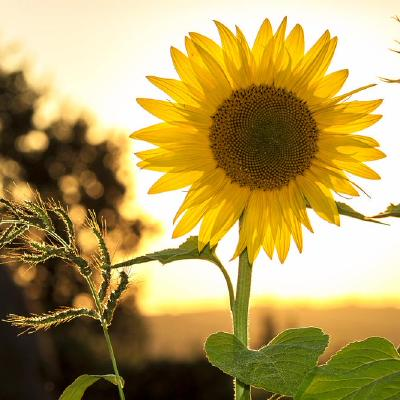
\includegraphics[width=\textwidth]{29571453}
  \caption{Figure caption here}
  \label{fig:29571453.jpg}
\end{figure}

\subsection{4.1.1 title}

\LaTeX\ commands are case-sensitive. Most are all lowercase. \LaTeX\ uses grouping to limit the effect of certain commands. Braces \{ ... \} are used to begin and end groups. For example, the
\textbackslash large command is usually used inside a group: \{\textbackslash large this is bigger than normal.\}  will produce {\large this is bigger than normal.} 

\LaTeX\ recognizes the following units:
\vskip 0.2in
\begin{tabular}{|c|c||c|c|}
  \hline 
  cm & centimeter & pt & printer’s point, $\approx$ 72 per inch \\ \hline
  mm & millimeter & em & font-dependent width of “m” \\ 	\hline
  in & inch & ex & font-dependent height of “x” \\ 	\hline
\end{tabular}
\vskip 0.2in

\chapter{Summary}
\null
\vfill

\noindent \Large{\textit{Look up at the stars and not down at your feet. Try to make sense of what you see and wonder about what makes the universe exist. Be curious.}}

\hfill \large{--Stephen Hawking}

\vspace{25mm} %20mm vertical space

\chapter*{Appendix}
\addcontentsline{toc}{chapter}{Appendix}

\renewcommand{\thesubsection}{\Alph{subsection}}
\renewcommand\linenumberfont{\normalfont\small}
\subsection{Appendix Subsection}

\lipsum[1]

\begin{linenumbers}
  \lipsum[2]
\end{linenumbers}

\lipsum[1]

\subsection*{Another appendix Subsection}

\addcontentsline{toc}{chapter}{Bibliography}
\bibliography{ref}{}
\bibliographystyle{unsrt}

\addcontentsline{toc}{chapter}{List of Figures}
\listoffigures

%\chapter*{List of Tables}
\addcontentsline{toc}{chapter}{List of Tables}
\listoftables

\chapter*{Curriculum vitae}
\addcontentsline{toc}{chapter}{Curriculum vitae}

\noindent Personal data

\noindent\rule{0.95\textwidth}{0.4pt}

\vskip 0.1in

\begin{tabular}{p{0.35\textwidth}p{0.55\textwidth}}
  Name: & San Zhang \\
  Date of birth: & 09.09.1999 \\
  Place of birth: & Beijing, China \\
\end{tabular} \\

\noindent Education

\noindent\rule{0.98\textwidth}{0.4pt}

\vskip 0.1in

\begin{tabular}{p{0.35\textwidth}p{0.55\textwidth}}
  09/2018-06/2022 & Bachelor, xxx University \\
  09/2022-06/2025 & Master, xxx University \\
  09/2025-08/2029 & Ph.D., xxx University \\
\end{tabular} \\

\end{document}
